\documentclass[11pt,a4paper]{article}

\usepackage[utf8]{inputenc}
\usepackage[T1]{fontenc}
\usepackage{amsmath,amssymb,amsthm}
\usepackage{booktabs}
\usepackage{graphicx}
\usepackage[margin=1in]{geometry}
\usepackage{hyperref}
\usepackage{xcolor}
\usepackage{fancyhdr}
\usepackage{float}
\usepackage{enumitem}
\usepackage{mathrsfs}

\graphicspath{{../figures/v2/}{figures/v2/}{../figures/}{figures/}}

\pagestyle{fancy}
\fancyhf{}
\fancyhead[C]{\small\itshape Quintuplets and the Sextuplet Boundary for $Q(n) = n^{47} - (n{-}1)^{47}$ --- Version 2}
\fancyfoot[C]{\thepage}
\renewcommand{\headrulewidth}{0.4pt}

\newtheorem{theorem}{Theorem}[section]
\newtheorem{lemma}[theorem]{Lemma}
\newtheorem{proposition}[theorem]{Proposition}
\newtheorem{corollary}[theorem]{Corollary}
\newtheorem{definition}[theorem]{Definition}
\newtheorem*{remark}{Remark}

\hypersetup{colorlinks=true, linkcolor=blue!60!black, citecolor=blue!60!black, urlcolor=blue!70!black}

\newcommand{\Sk}[1]{\mathfrak{S}_{#1}}

\title{\textbf{Prime Quintuplets and the Sextuplet Boundary} \\[6pt]
\textbf{for} $\boldsymbol{Q(n) = n^{47} - (n-1)^{47}}$ \\[6pt]
\large Extreme Prime Clusters in a High-Degree Polynomial \\[4pt]
\normalsize Version 2 (revised and corrected)}

\author{Ruqing Chen \\[4pt]
\textit{GUT Geoservice Inc., Montr\'eal, Canada} \\
\texttt{ruqing@hotmail.com}}

\date{October 2026 (Version 2; Version 1: February 2026) \\[6pt]
\normalsize DOI: \href{https://doi.org/10.5281/zenodo.23178170}{10.5281/zenodo.23178170} (Version 2)
\quad $\cdot$ \quad
\href{https://doi.org/10.5281/zenodo.18728917}{10.5281/zenodo.18728917} (Version 1)}

\begin{document}
\maketitle
\thispagestyle{fancy}

\begin{center}
\textit{Subject: Analytic Number Theory / Computational Mathematics} \\[4pt]
\textit{Part III of the Titan Project}
\end{center}

\begin{abstract}
Among the 742 prime quadruplets found for
$Q(n) = n^{47} - (n{-}1)^{47}$ over $1 \leq n \leq 2 \times 10^{11}$
\cite{Chen2026b}, exactly \textbf{7 extend to prime quintuplets}
(five consecutive integers all generating probable primes of
488--520 digits), while \textbf{no sextuplet} was found.
This paper develops a quantitative theory for this emergence--extinction
transition.

$Q(n)$ is the homogenised 47th cyclotomic polynomial $\Phi_{47}(n, n{-}1)$.
Consequently every prime divisor of every value $Q(n)$ is congruent to
$1 \pmod{47}$, and the root count is \emph{bifurcated}:
$\omega_1(p) = 0$ for $p \not\equiv 1 \pmod{47}$ and
$\omega_1(p) = 46$ for the \emph{resonant primes} $p \equiv 1 \pmod{47}$.
The resonant primes impose a periodic sieve obstruction that produces
``cliffs'' in the Bateman--Horn Euler product, the first at $p = 283$.
Because the plain Euler product converges only conditionally (it still
oscillates by $\pm 20\%$ for sieve bounds up to $10^4$), we evaluate the
singular series \emph{exactly} by factoring out the Dirichlet $L$-values
$\prod_{\chi \neq \chi_0} L(1,\chi) = 0.1151693$ modulo~47, which leaves an
absolutely convergent product.  This gives
$\Sk{4} = 6{,}514$, $\Sk{5} = 58{,}550$ and $\Sk{6} = 535{,}500$
with no calibration to the data.
The resulting parameter-free predictions,
$E[C_4] = 747$, $E[C_5] = 5.9$ and $E[C_6] = 0.047$ at $N = 2 \times 10^{11}$,
agree with the observed 749 quadruplet positions, 7 quintuplets and 0 sextuplets;
in the pioneer zone ($N = 2 \times 10^9$) the predicted numbers of primes
and prime pairs agree with the census to $0.05\%$ and $0.07\%$.
The first sextuplet is predicted at
$\boldsymbol{N^* \approx 1.0 \times 10^{13}}$,
a ${\sim}50$-fold extension of the present search, where the primes have
${\sim}601$ digits.  The inter-level suppression factor is not a constant:
it equals $(I_k/I_{k+1})/(\Sk{k+1}/\Sk{k}) \approx 46\ln N / 9$, i.e.\
${\approx}103$ at $N = 2 \times 10^9$ and ${\approx}127$ at $N = 2 \times 10^{11}$,
which reconciles the pioneer-zone ratios with the full-range one.

\medskip
\noindent\textbf{Keywords:}
prime quintuplets, sextuplet boundary, Bateman--Horn conjecture,
singular series, cyclotomic polynomial, resonant primes, Dirichlet $L$-functions,
constellation hierarchy, high-degree polynomials

\medskip
\noindent\textbf{MSC 2020:} 11N32, 11A41, 11Y11, 11Y16, 11M20, 11R18
\end{abstract}

\paragraph{Changes in Version 2.}
Version 1 \cite{Chen2026c} tabulated partial Euler products that, except at the
sieve bound $B = 10^4$, were not the output of the published script; the
convergence claim based on a ``calibration factor of 0.999'' was therefore
unsupported.  Version 2 replaces that table with the correct partial products
(Table~\ref{tab:singular}), adds an exact $L$-function evaluation of the singular
series (Section~\ref{sec:exact}), removes the empirical calibration, corrects the
digit counts of the quintuplets (each was one too small), corrects the
Kolmogorov--Smirnov statistic, the prime count in the ``unobstructed corridor'',
the Poisson interval, the cost estimate, and replaces the claim of a constant
suppression factor by the correct $\ln N$ dependence.  A complete list is given in
\texttt{CHANGELOG\_v2.md} in the data repository.

%==========================================================================
\section{Introduction}
%==========================================================================

A \emph{prime $k$-constellation} of the polynomial
$Q(n) = n^{47} - (n{-}1)^{47}$ is a run of~$k$ consecutive integers
$n, n{+}1, \ldots, n{+}k{-}1$ such that all~$k$ values of~$Q$ are
(probable) primes.  The census of the pioneer zone
($n \leq 2 \times 10^9$)~\cite{Chen2026a} established a strict
morphological hierarchy---18.1~million solitary primes, 173{,}351~pairs,
1{,}749~triplets, 15~quadruplets---with inter-level ratios
of approximately $100{\times}$.  The deep-space census~\cite{Chen2026b}
extended the quadruplet search to $N = 2 \times 10^{11}$, finding
742~quadruplets, 7 of which are quintuplets, and zero sextuplets.

The present paper (Part~III of the Titan Project) addresses the
central question arising from these data:
\begin{quote}
\itshape Why do exactly 7 quintuplets emerge from 742 quadruplets,
and why does the sextuplet order remain vacant across 200~billion integers?
\end{quote}
We answer it through:
\begin{enumerate}[label=(\roman*)]
  \item The identification of $Q(n)$ with the homogenised cyclotomic polynomial
    $\Phi_{47}(n, n{-}1)$, which gives the \emph{bifurcated root structure}:
    zero roots for most primes, but exactly 46 roots modulo every
    prime $p \equiv 1 \pmod{47}$ (the \emph{resonant primes});
  \item An \emph{exact} evaluation of the singular series
    $\Sk{1}, \ldots, \Sk{6}$ by factoring out the Dirichlet $L$-values
    modulo~47, together with the (slowly, conditionally convergent) plain
    Euler products for comparison;
  \item A parameter-free Bateman--Horn validation across the whole
    hierarchy, from 18~million primes down to 7 quintuplets;
  \item A quantitative prediction for the sextuplet boundary at
    $N^* \approx 1.0 \times 10^{13}$;
  \item Analysis of the spatial distribution of the 7 quintuplets and of the
    $N$-dependence of the inter-level suppression factor.
\end{enumerate}

\subsection{Counting conventions}

The Bateman--Horn conjecture~\cite{BatemanHorn1962} predicts the number of
\emph{positions} $n \leq N$ such that the $k$ values
$Q(n), \ldots, Q(n{+}k{-}1)$ are all prime:
\begin{equation}\label{eq:BH}
  C_k(N) \;\sim\; \Sk{k}\, I_k(N), \qquad
  I_k(N) = \int_2^N \frac{dt}{\prod_{i=0}^{k-1} \ln Q(t{+}i)}
  \approx \int_2^N \frac{dt}{(46 \ln t + \ln 47)^k}\,,
\end{equation}
since $Q(t) = 47t^{46} - \binom{47}{2} t^{45} + \cdots$.  Version~1 used
$(46 \ln t)^k$ in the denominator; the $\ln 47$ term lowers $I_4$ by $1.3\%$
and $I_6$ by $2.0\%$ at $N = 2 \times 10^{11}$ and is kept throughout this
version.  A census, on the other hand, reports \emph{maximal runs}: a
quintuplet is listed once, not also as two quadruplets.  A maximal run of
length~$m$ contains $m{-}k{+}1$ positions of order~$k$, so the 742 quadruplets
of Part~II (735 of exact length~4 plus the 7 quintuplets) correspond to
$735 + 2 \times 7 = 749$ quadruplet positions.  All comparisons with
\eqref{eq:BH} below use position counts.

%==========================================================================
\section{The Bifurcated Root Structure of $Q(n)$}\label{sec:roots}
%==========================================================================

\subsection{$Q(n)$ as a cyclotomic value}

Since $x^{47} - 1 = (x-1)\Phi_{47}(x)$ with $\Phi_{47}(x) = x^{46} + \cdots + 1$,
\begin{equation}\label{eq:cyclo}
  Q(n) = n^{47} - (n{-}1)^{47}
       = \bigl(n - (n{-}1)\bigr)\,(n{-}1)^{46}\,\Phi_{47}\!\Bigl(\frac{n}{n{-}1}\Bigr)
       = \Phi_{47}(n,\, n{-}1),
\end{equation}
the homogenised 47th cyclotomic polynomial evaluated at the coprime pair
$(n, n{-}1)$.  It is irreducible of degree~46 with leading coefficient~47.
A classical theorem on the divisors of $a^q - b^q$
\cite{BirkhoffVandiver1904,Washington1997} states that every prime divisor
of $\Phi_q(a,b)$ with $\gcd(a,b) = 1$ and $q$ prime is either $q$ itself or
congruent to $1 \pmod q$.  Because $n^{47} \equiv n \pmod{47}$ by Fermat,
$Q(n) \equiv n - (n{-}1) = 1 \pmod{47}$, so $47$ never divides $Q(n)$.  Hence:

\begin{proposition}\label{prop:divisors}
Every prime factor of every value $Q(n)$, $n \geq 2$, is congruent to
$1 \pmod{47}$.  In particular $Q(n)$ is odd, prime to~$3$, and prime to every
prime $< 283$.
\end{proposition}

\subsection{Main Theorem}

\begin{theorem}[Bifurcated Root Structure]\label{thm:roots}
Let $p$ be a prime and $Q(n) = n^{47} - (n{-}1)^{47}$.  Then:
\begin{enumerate}[label=(\alph*)]
  \item If $p \nmid n(n{-}1)$, then $Q(n) \equiv 0 \pmod{p}$
    if and only if $n/(n{-}1)$ is a nontrivial 47th root of unity modulo~$p$.
    Such roots exist if and only if $p \equiv 1 \pmod{47}$.
  \item If $p \mid n$ or $p \mid (n{-}1)$, then $Q(n) \equiv 1 \pmod{p}$.
  \item \textbf{Root count:}
    \begin{equation}\label{eq:rootcount}
      \omega_1(p) =
      \begin{cases}
        46 & \text{if } p \equiv 1 \pmod{47}, \\
        0  & \text{otherwise.}
      \end{cases}
    \end{equation}
\end{enumerate}
\end{theorem}

\begin{proof}
\textbf{(a)}  Suppose $p \nmid n(n{-}1)$ and write $a = n$, $b = n{-}1$.
Then $Q(n) \equiv 0$ iff $(a/b)^{47} \equiv 1 \pmod{p}$.
Let $g = \gcd(47, p{-}1) \in \{1, 47\}$.
If $g = 1$ the only solution of $x^{47} = 1$ in $\mathbb{F}_p^*$ is $x = 1$,
forcing $a \equiv b$, i.e.\ $1 \equiv 0$---impossible; so $\omega_1(p) = 0$.
If $g = 47$ then $p \equiv 1 \pmod{47}$ and $\mathbb{F}_p^*$ contains a cyclic
subgroup of order~47 generated by $\zeta = g_0^{(p-1)/47}$, $g_0$ a primitive root.
For each $j \in \{1, \ldots, 46\}$ the equation $a/b = \zeta^j$ with $a = b + 1$
gives $b(\zeta^j - 1) = 1$, hence the unique root
\begin{equation}\label{eq:roots}
  n_j = 1 + (\zeta^j - 1)^{-1} \pmod p, \qquad j = 1, \ldots, 46,
\end{equation}
and these 46 residues are distinct because $j \mapsto \zeta^j$ is injective.
Both $b$ and $a = \zeta^j b$ are units, so no root is lost to the excluded cases.
\textbf{(b)}  If $p \mid n$ then $Q(n) \equiv -(-1)^{47} = 1$; if $p \mid (n{-}1)$
then $Q(n) \equiv 1^{47} - 0 = 1$.
\end{proof}

Theorem~\ref{thm:roots} is the statement that $\Phi_{47}$ splits completely
modulo~$p$ exactly when $p$ splits completely in $\mathbb{Q}(\zeta_{47})$,
i.e.\ when $p \equiv 1 \pmod{47}$; since $Q$ has degree~46, resonant primes
carry the maximal possible number of roots.

\paragraph{Explicit example.}
The smallest resonant prime is $p = 283 = 6 \times 47 + 1$.
A primitive 47th root of unity is $\zeta = 2^{6} = 64$
(indeed $64 \neq 1$ and $64^{47} \equiv 1 \pmod{283}$).
For $j = 1$: $b = 63^{-1} \equiv 9 \pmod{283}$ since $63 \times 9 = 567 = 2 \times 283 + 1$;
thus $n_1 = 10$ and $Q(10) = 10^{47} - 9^{47} \equiv 0 \pmod{283}$.
Direct enumeration confirms exactly 46 roots modulo~283.

\subsection{Resonant Primes and the Periodic Sieve Obstruction}

\begin{definition}[Resonant Primes]
A prime $p$ is \emph{resonant} for $Q$ if $p \equiv 1 \pmod{47}$:
$\mathcal{R} = \{283, 659, 941, 1129, 1223, 1693, \ldots\}$.
By Dirichlet's theorem a proportion $1/\varphi(47) = 1/46$ of all primes is
resonant; there are 28 resonant primes below $10^4$ (Dirichlet expectation 26.7)
and 1{,}700 below $10^6$ (expectation 1{,}706).
\end{definition}

For $k$-constellations the relevant quantity is $\omega_k(p)$, the number of
residues~$r$ modulo~$p$ for which at least one of $Q(r), \ldots, Q(r{+}k{-}1)$
vanishes.  By \eqref{eq:roots} this is the size of the union of the $k$ shifted
root sets $\{n_j - i\}$, $0 \leq i < k$.  Two shifted sets overlap only if
$n_j - n_{j'} \equiv d \pmod p$ for some $d \in \{\pm 1, \ldots, \pm(k{-}1)\}$,
which happens only for primes dividing the norm of the algebraic number
$(\zeta^j-1)^{-1} - (\zeta^{j'}-1)^{-1} - d \in \mathbb{Q}(\zeta_{47})$---a
finite set of primes for each $k$.  Hence
\begin{equation}\label{eq:omegak}
  \omega_k(p) = 46k \quad\text{for all but finitely many resonant } p,
  \qquad \omega_k(p) = 0 \quad\text{for non-resonant } p .
\end{equation}
Below $10^4$ the exceptional resonant primes for $k = 6$ are
283, 659, 941, 1129, 1223, 1693, 1787, 2069, 2351, 2539, 2633, 3761, 4513,
4889, 5077, 5171, 6863 and 8461; from $p = 5641$ on, all but 6863 and 8461
attain $\omega_6 = 276$.  Table~\ref{tab:omega} lists the first five resonant primes.

\begin{table}[H]
\centering
\caption{Root counts $\omega_k(p)$ at the first five resonant primes and the
local Bateman--Horn factors $\sigma_k(p) = (1 - \omega_k/p)/(1 - 1/p)^k$.
For non-resonant primes $\omega_k = 0$ and $\sigma_k(p) = (p/(p{-}1))^k$.}\label{tab:omega}
\smallskip
\begin{tabular}{crrrrrrccc}
\toprule
$p$ & $\omega_1$ & $\omega_2$ & $\omega_3$ & $\omega_4$ & $\omega_5$ & $\omega_6$ &
  $\sigma_4(p)$ & $\sigma_5(p)$ & $\sigma_6(p)$ \\
\midrule
283  & 46 & 78 & 102 & 126 & 148 & 164 & 0.563 & 0.486 & 0.430 \\
659  & 46 & 88 & 124 & 160 & 194 & 228 & 0.762 & 0.711 & 0.660 \\
941  & 46 & 92 & 134 & 176 & 216 & 256 & 0.816 & 0.775 & 0.733 \\
1129 & 46 & 88 & 128 & 166 & 202 & 235 & 0.856 & 0.825 & 0.796 \\
1223 & 46 & 88 & 125 & 162 & 195 & 226 & 0.870 & 0.844 & 0.819 \\
\midrule
generic $p \in \mathcal{R}$ & 46 & 92 & 138 & 184 & 230 & 276 &
  \multicolumn{3}{c}{$\approx 1 - 45k/p$} \\
\bottomrule
\end{tabular}
\end{table}

The first resonant prime $p = 283$ is the most destructive:
$\sigma_4(283) = 0.563$ nearly halves the running Euler product for quadruplets
(Figure~\ref{fig:euler}).  Subsequent resonant primes produce progressively milder
corrections as $\omega_k/p \to 0$.  The 60 primes below 283 all have
$\omega_k = 0$ (Proposition~\ref{prop:divisors}); this ``unobstructed corridor''
lets the product climb to $\Sk{4}(282) = 10{,}780$ before the first cliff and is
the reason for the large absolute size of the constants.

%==========================================================================
\section{Computing the Singular Series}\label{sec:singular}
%==========================================================================

\subsection{Plain Euler products}

The Bateman--Horn singular series for $k$-constellations is
\begin{equation}\label{eq:Sk}
  \Sk{k} = \prod_{p} \sigma_k(p), \qquad
  \sigma_k(p) = \frac{1 - \omega_k(p)/p}{(1 - 1/p)^k}.
\end{equation}
With \eqref{eq:omegak}, $\ln \sigma_k(p) \approx (k - \omega_k(p))/p$, which is
$+k/p$ at the 45 out of 46 non-resonant primes and $\approx -45k/p$ at each
resonant prime.  The two contributions cancel \emph{on average}, so the product
converges, but only conditionally: between consecutive resonant primes the
partial product climbs by a factor $\approx (\ln p'/\ln p)^k$ and then drops by
$1 - 46k/p$.  Table~\ref{tab:singular} and Figure~\ref{fig:convergence} show
this saw-tooth.  Even at $B = 10^4$ the partial product is still $2$--$3\%$
below its limit, and at $B = 10^5$ it is $0.7$--$1.0\%$ above it; a truncated
product cannot certify its own convergence.

\begin{table}[H]
\centering
\caption{Plain partial singular series $\Sk{k}(B) = \prod_{p \le B} \sigma_k(p)$,
computed with the exact root counts (script
\texttt{compute\_singular\_series\_v2.py}; the $B = 10^4$ row is also produced by
the Version~1 script).  Last row: exact values from Section~\ref{sec:exact}.}
\label{tab:singular}
\smallskip
\begin{tabular}{lrrrl}
\toprule
Sieve bound $B$ & $\Sk{4}(B)$ & $\Sk{5}(B)$ & $\Sk{6}(B)$ & Note \\
\midrule
100     &  4{,}772 &  39{,}661 &   329{,}634 & no resonant prime yet \\
282     & 10{,}780 & 109{,}847 & 1{,}119{,}303 & just before the first cliff \\
283     &  6{,}066 &  53{,}336 &   480{,}764 & first cliff ($\times 0.563$, $0.486$, $0.430$) \\
1{,}000 &  7{,}947 &  74{,}537 &   710{,}658 & partial recovery \\
5{,}000 &  6{,}668 &  60{,}315 &   555{,}276 & \\
$10^4$  &  6{,}392 &  57{,}173 &   520{,}348 & Version-1 truncation point \\
$10^5$  &  6{,}559 &  59{,}045 &   540{,}940 & \\
$10^6$  &  6{,}502 &  58{,}410 &   533{,}966 & \\
\midrule
\textbf{Exact} & \textbf{6{,}514} & \textbf{58{,}550} & \textbf{535{,}502} &
  $L$-function evaluation, Eq.~\eqref{eq:accel} \\
\bottomrule
\end{tabular}
\end{table}

\begin{figure}[htbp]
\centering
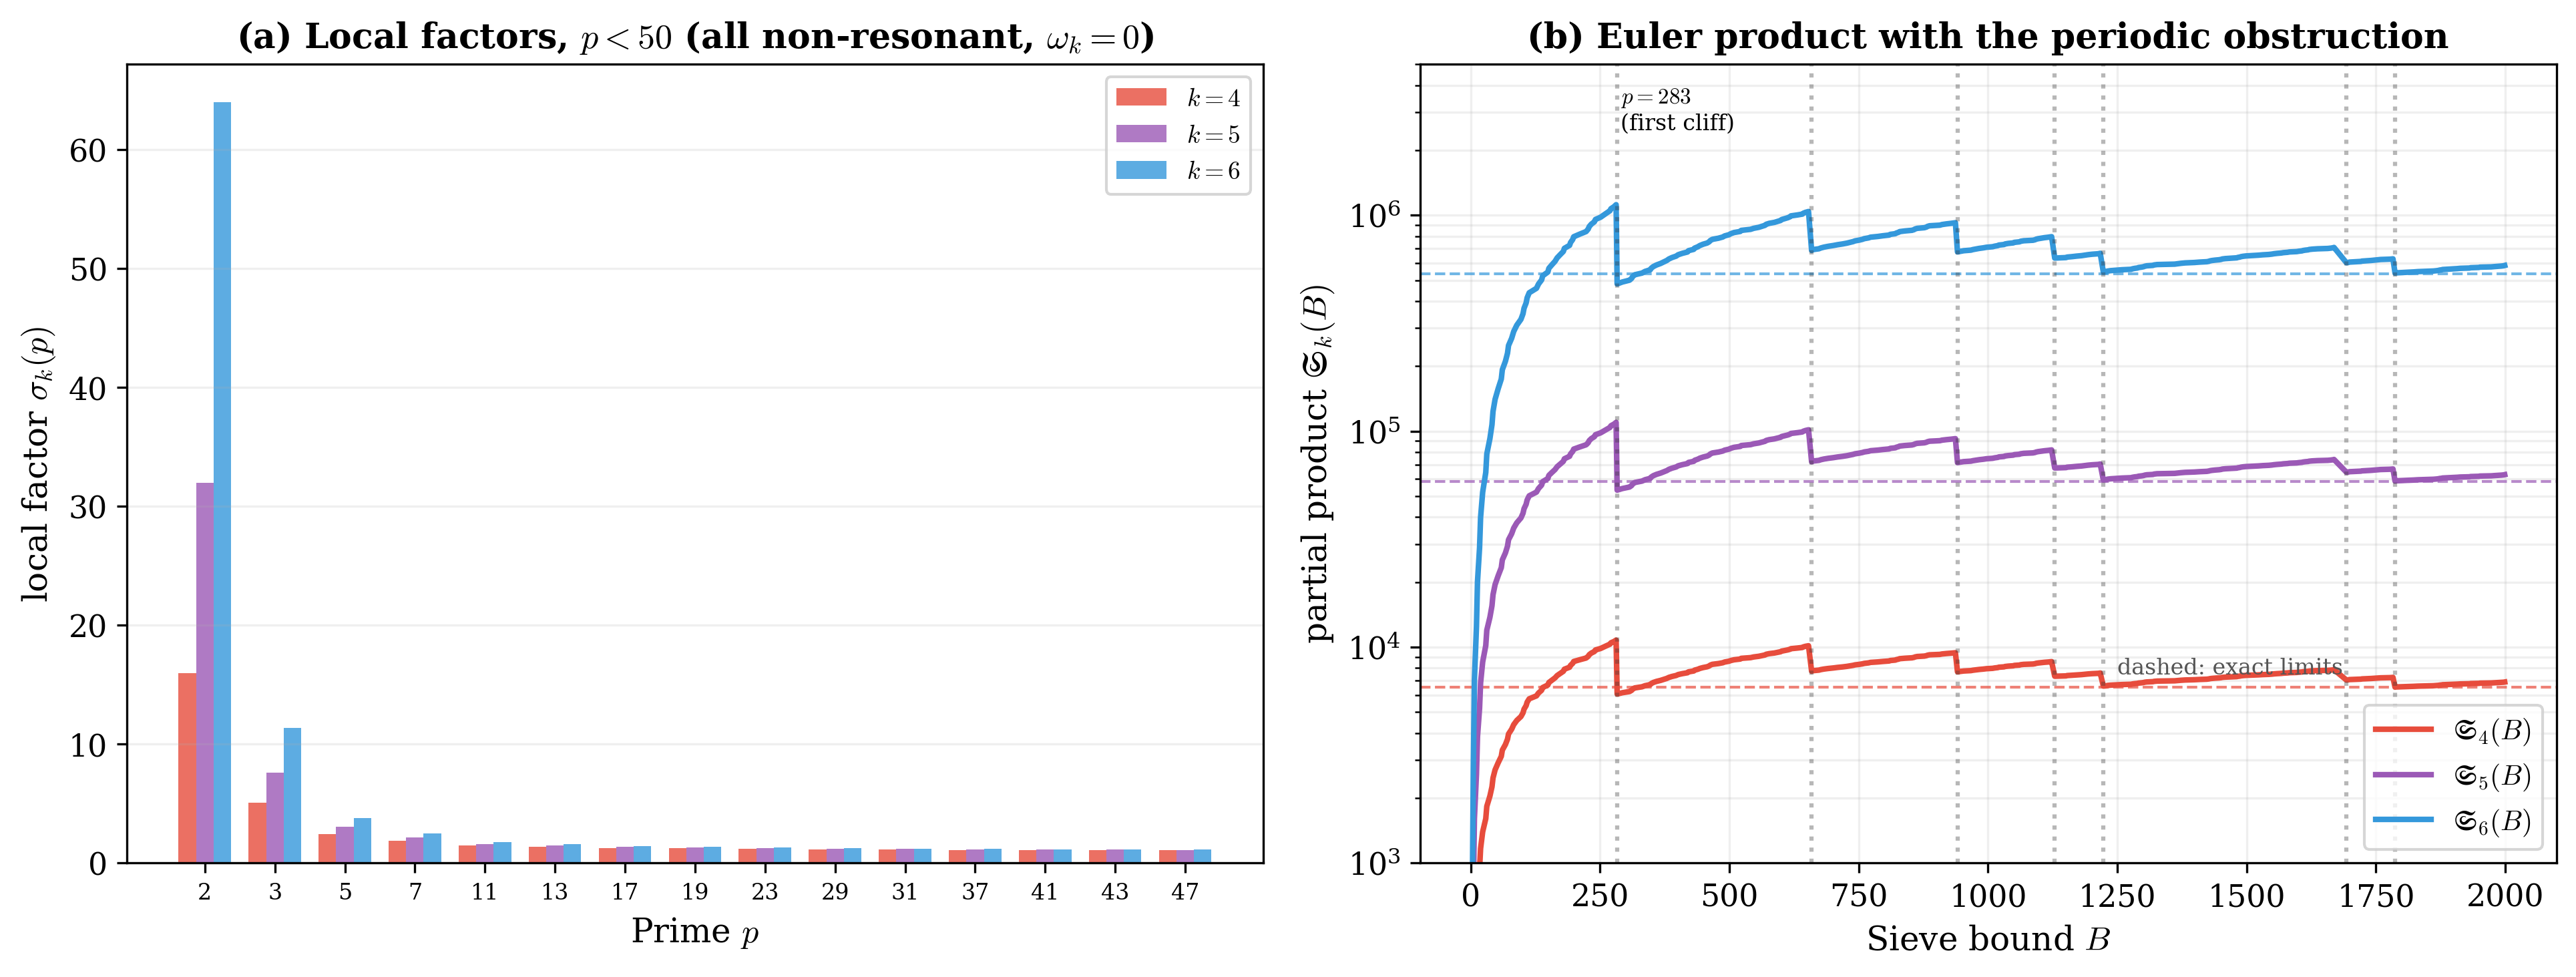
\includegraphics[width=\textwidth]{v2_fig4.png}
\caption{(a)~Local factors for the non-resonant primes $p < 50$:
$\sigma_k(p) = (p/(p{-}1))^k$.
(b)~Partial products $\Sk{k}(B)$ for $B \le 2000$, showing the cliff at
$p = 283$ and the subsequent saw-tooth; dashed lines are the exact
values.}\label{fig:euler}
\end{figure}

\subsection{Exact evaluation via Dirichlet $L$-functions}\label{sec:exact}

Let $\chi$ run over the 45 non-principal Dirichlet characters modulo~47 (all
primitive) and let $f = f(p)$ denote the order of $p$ modulo~47, so that
$\prod_{\chi \neq \chi_0}(1 - \chi(p)/p) = (1 - p^{-f})^{46/f}/(1 - 1/p)$ for
$p \neq 47$.  Multiplying and dividing \eqref{eq:Sk} by
$\prod_{\chi \ne \chi_0} L(1,\chi)^{k}$ gives
\begin{equation}\label{eq:accel}
\begin{aligned}
  \Sk{k} &= \Bigl[\prod_{\chi \neq \chi_0} L(1,\chi)\Bigr]^{-k}
           \prod_{p} B_k(p), \\
  B_k(p) &= \Bigl(1 - \frac{\omega_k(p)}{p}\Bigr)\bigl(1 - p^{-f}\bigr)^{-46k/f}
  \quad (p \ne 47), \qquad B_k(47) = \Bigl(\frac{47}{46}\Bigr)^{k}.
\end{aligned}
\end{equation}
For a generic resonant prime ($f = 1$, $\omega_k = 46k$) one has
$B_k(p) = (1 - 46k/p)(1 - 1/p)^{-46k} = 1 + O(k^2/p^2)$, and for a
non-resonant prime ($f \geq 2$) $B_k(p) = 1 + O(k/p^2)$.  The product in
\eqref{eq:accel} is therefore absolutely convergent, with tail
$O\bigl(k^2/(B \ln B)\bigr)$ beyond a cut-off $B$.  The $L$-values are computed
exactly from the finite formulas for primitive characters
\cite[Thm.~4.9]{Washington1997}; the quadratic character gives the check
$L(1,\chi_{47}) = \pi h(-47)/\sqrt{47} = 2.29124\ldots$ with $h(-47) = 5$, and
\begin{equation}
  \prod_{\chi \neq \chi_0 \ (\mathrm{mod}\ 47)} L(1,\chi) = 0.115169277\ldots,
\end{equation}
which by the analytic class number formula is the residue of the Dedekind zeta
function of $\mathbb{Q}(\zeta_{47})$ at $s = 1$.

\begin{table}[H]
\centering
\caption{Convergence of the accelerated product \eqref{eq:accel} with the cut-off~$B$.}
\label{tab:accel}
\smallskip
\begin{tabular}{lrrrrrr}
\toprule
$B$ & $\Sk{1}$ & $\Sk{2}$ & $\Sk{3}$ & $\Sk{4}$ & $\Sk{5}$ & $\Sk{6}$ \\
\midrule
$10^3$ & 8.7146 & 78.341 & 724.56 & 6{,}535.9 & 58{,}377 & 530{,}038 \\
$10^4$ & 8.6846 & 77.990 & 722.74 & 6{,}527.4 & 58{,}688 & 536{,}938 \\
$10^5$ & 8.6829 & 77.945 & 721.92 & 6{,}514.7 & 58{,}552 & 535{,}529 \\
$10^6$ & 8.6827 & 77.943 & 721.90 & 6{,}514.5 & 58{,}550 & 535{,}502 \\
$3 \times 10^6$ & 8.6827 & 77.943 & 721.89 & 6{,}514.4 & 58{,}549 & 535{,}495 \\
\bottomrule
\end{tabular}
\end{table}

We adopt
\begin{equation}\label{eq:values}
  \Sk{1} = 8.683,\quad \Sk{2} = 77.94,\quad \Sk{3} = 721.9,\quad
  \Sk{4} = 6{,}514,\quad \Sk{5} = 58{,}550,\quad \Sk{6} = 535{,}500,
\end{equation}
accurate to about $10^{-4}$ relative, and the inter-level ratios
\begin{equation}\label{eq:ratios}
  \frac{\Sk{2}}{\Sk{1}} = 8.98,\quad
  \frac{\Sk{3}}{\Sk{2}} = 9.26,\quad
  \frac{\Sk{4}}{\Sk{3}} = 9.02,\quad
  \frac{\Sk{5}}{\Sk{4}} = 8.99,\quad
  \frac{\Sk{6}}{\Sk{5}} = 9.15,\quad
  \frac{\Sk{6}}{\Sk{4}} = 82.2 .
\end{equation}
The ratios are all close to~9, the value $\prod_{\chi\neq\chi_0}L(1,\chi)^{-1} \approx 8.68$
corrected by the overlap of shifted root sets at the small resonant primes.
(Version~1 compared these ratios with ``root-free'' values; since the root-free
product $\prod_{p \le B}(1-1/p)^{-k}$ diverges like $(e^\gamma \ln B)^k$, that
comparison has no limit and is withdrawn.)

\begin{figure}[htbp]
\centering
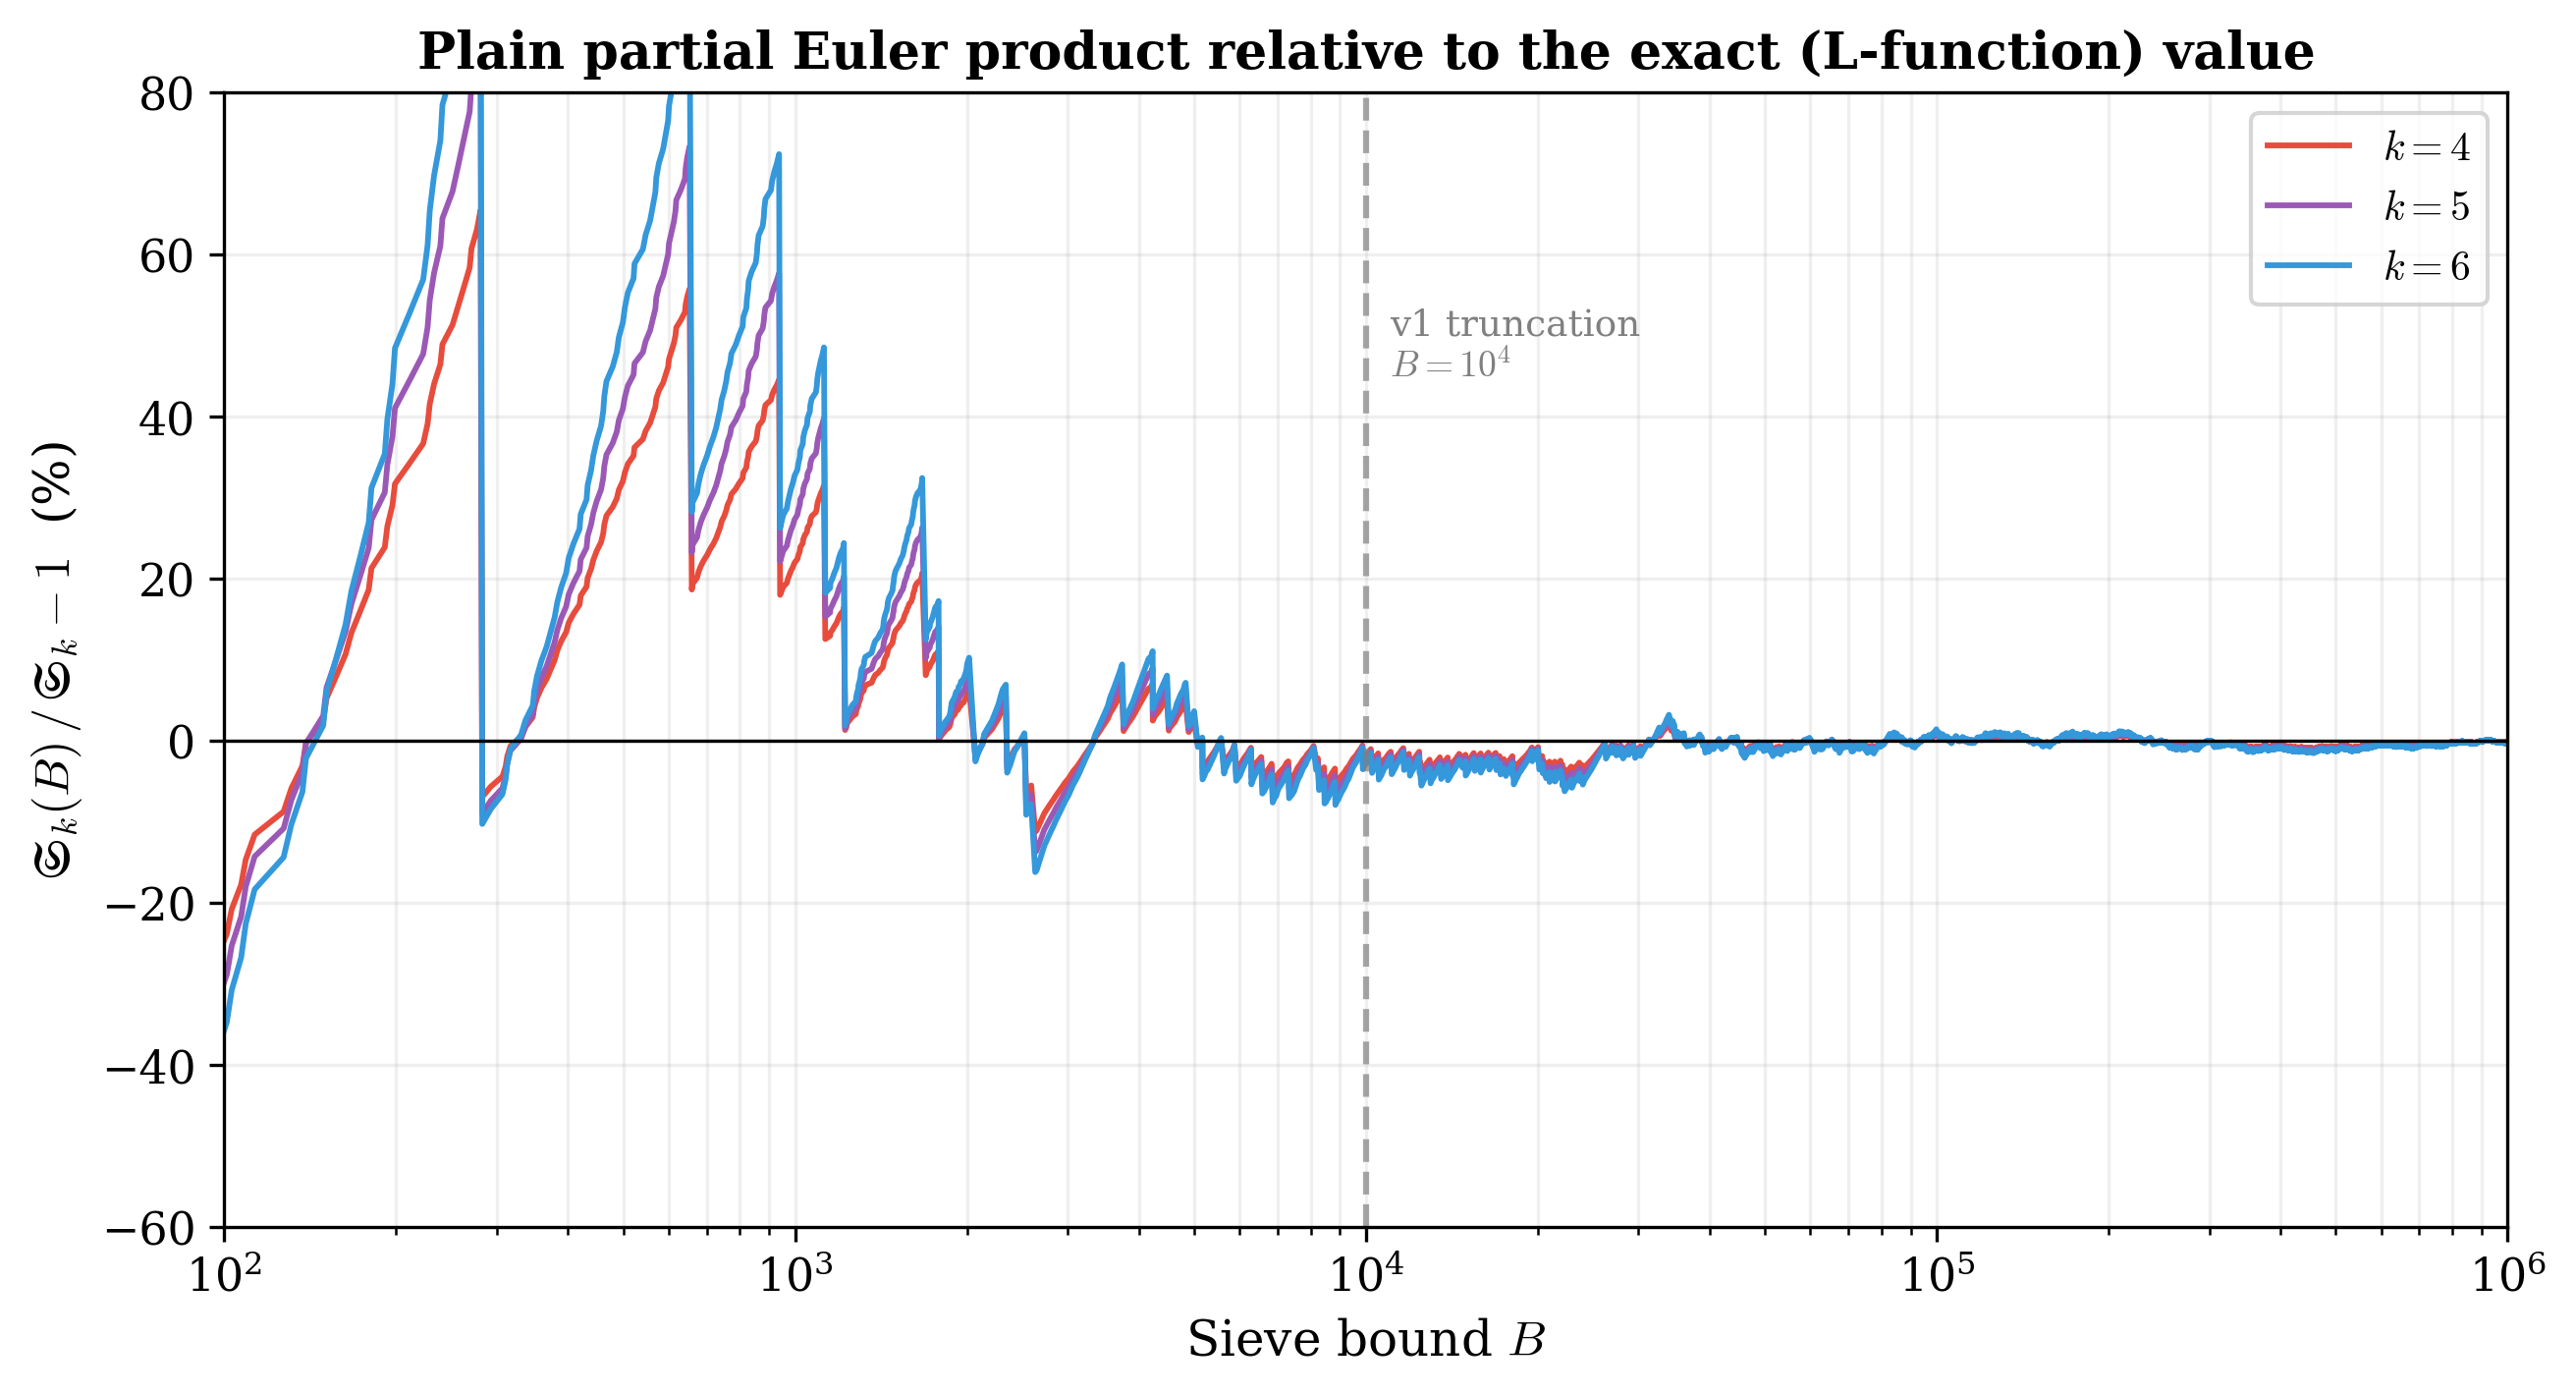
\includegraphics[width=0.95\textwidth]{v2_fig5.png}
\caption{Relative deviation of the plain partial product $\Sk{k}(B)$ from the
exact value, for $k = 4, 5, 6$ and $B \le 10^6$.  The oscillation is
$\pm 20\%$ at $B \sim 10^3$ and still $\pm 1\%$ at $B \sim 10^5$; the Version-1
truncation at $B = 10^4$ happened to fall within $3\%$ of the limit.}
\label{fig:convergence}
\end{figure}

\subsection{Parameter-free validation across the hierarchy}\label{sec:validation}

With \eqref{eq:values} and \eqref{eq:BH}, Bateman--Horn gives predictions
without any fitted quantity.  Table~\ref{tab:hierarchy} compares them with the
two censuses, converting maximal-run counts to position counts as explained in
Section~1.1.\footnote{The pioneer-zone categories of Part~I are read as runs of
exact length (``solitary'' = isolated prime, ``pair'' = exactly two consecutive
primes, etc.).  Under this reading the total number of primes is
$18{,}121{,}562 + 2 \times 173{,}351 + 3 \times 1{,}749 + 4 \times 15 = 18{,}473{,}571$.
If instead ``solitary'' meant all primes, the deviation would be $-1.9\%$
(80 standard deviations), so the data themselves fix the convention.}

\begin{table}[H]
\centering
\caption{Bateman--Horn predictions with the exact singular series versus the
observed position counts.  Deviations are in units of the Poisson standard
deviation $\sqrt{E}$.}\label{tab:hierarchy}
\smallskip
\begin{tabular}{clrrrr}
\toprule
$N$ & $k$ & Census (as reported) & Positions & $E[C_k(N)]$ & Deviation \\
\midrule
$2\times 10^{9}$  & 1 & 18{,}121{,}562 & 18{,}473{,}571 & 18{,}464{,}404 & $+0.05\%$ ($+2.1\sigma$) \\
$2\times 10^{9}$  & 2 &    173{,}351 &    176{,}894 &    176{,}778 & $+0.07\%$ ($+0.3\sigma$) \\
$2\times 10^{9}$  & 3 &      1{,}749 &      1{,}779 &      1{,}752 & $+1.5\%$ ($+0.6\sigma$) \\
$2\times 10^{9}$  & 4 &           15 &           15 &         17.0 & $-0.5\sigma$ \\
$2\times 10^{11}$ & 4 &          742 &          749 &        746.9 & $+0.3\%$ ($+0.1\sigma$) \\
$2\times 10^{11}$ & 5 &            7 &            7 &         5.88 & $+0.5\sigma$ \\
$2\times 10^{11}$ & 6 &            0 &            0 &        0.047 & $-0.2\sigma$ \\
\bottomrule
\end{tabular}
\end{table}

The agreement at $k = 1$ and $k = 2$---five and three significant figures
respectively---is the strongest evidence that the singular series
\eqref{eq:values} and the integral \eqref{eq:BH} are correct in detail.  The
empirical constant $749/I_4(2 \times 10^{11}) = 6{,}533$ agrees with the exact
$\Sk{4} = 6{,}514$ to $0.3\%$, well inside the $3.7\%$ Poisson uncertainty of a
count of~749; Version~1's calibrated value $6{,}385$ was lower only because it
used $(46\ln t)^4$ and the run count 742.

\begin{figure}[htbp]
\centering
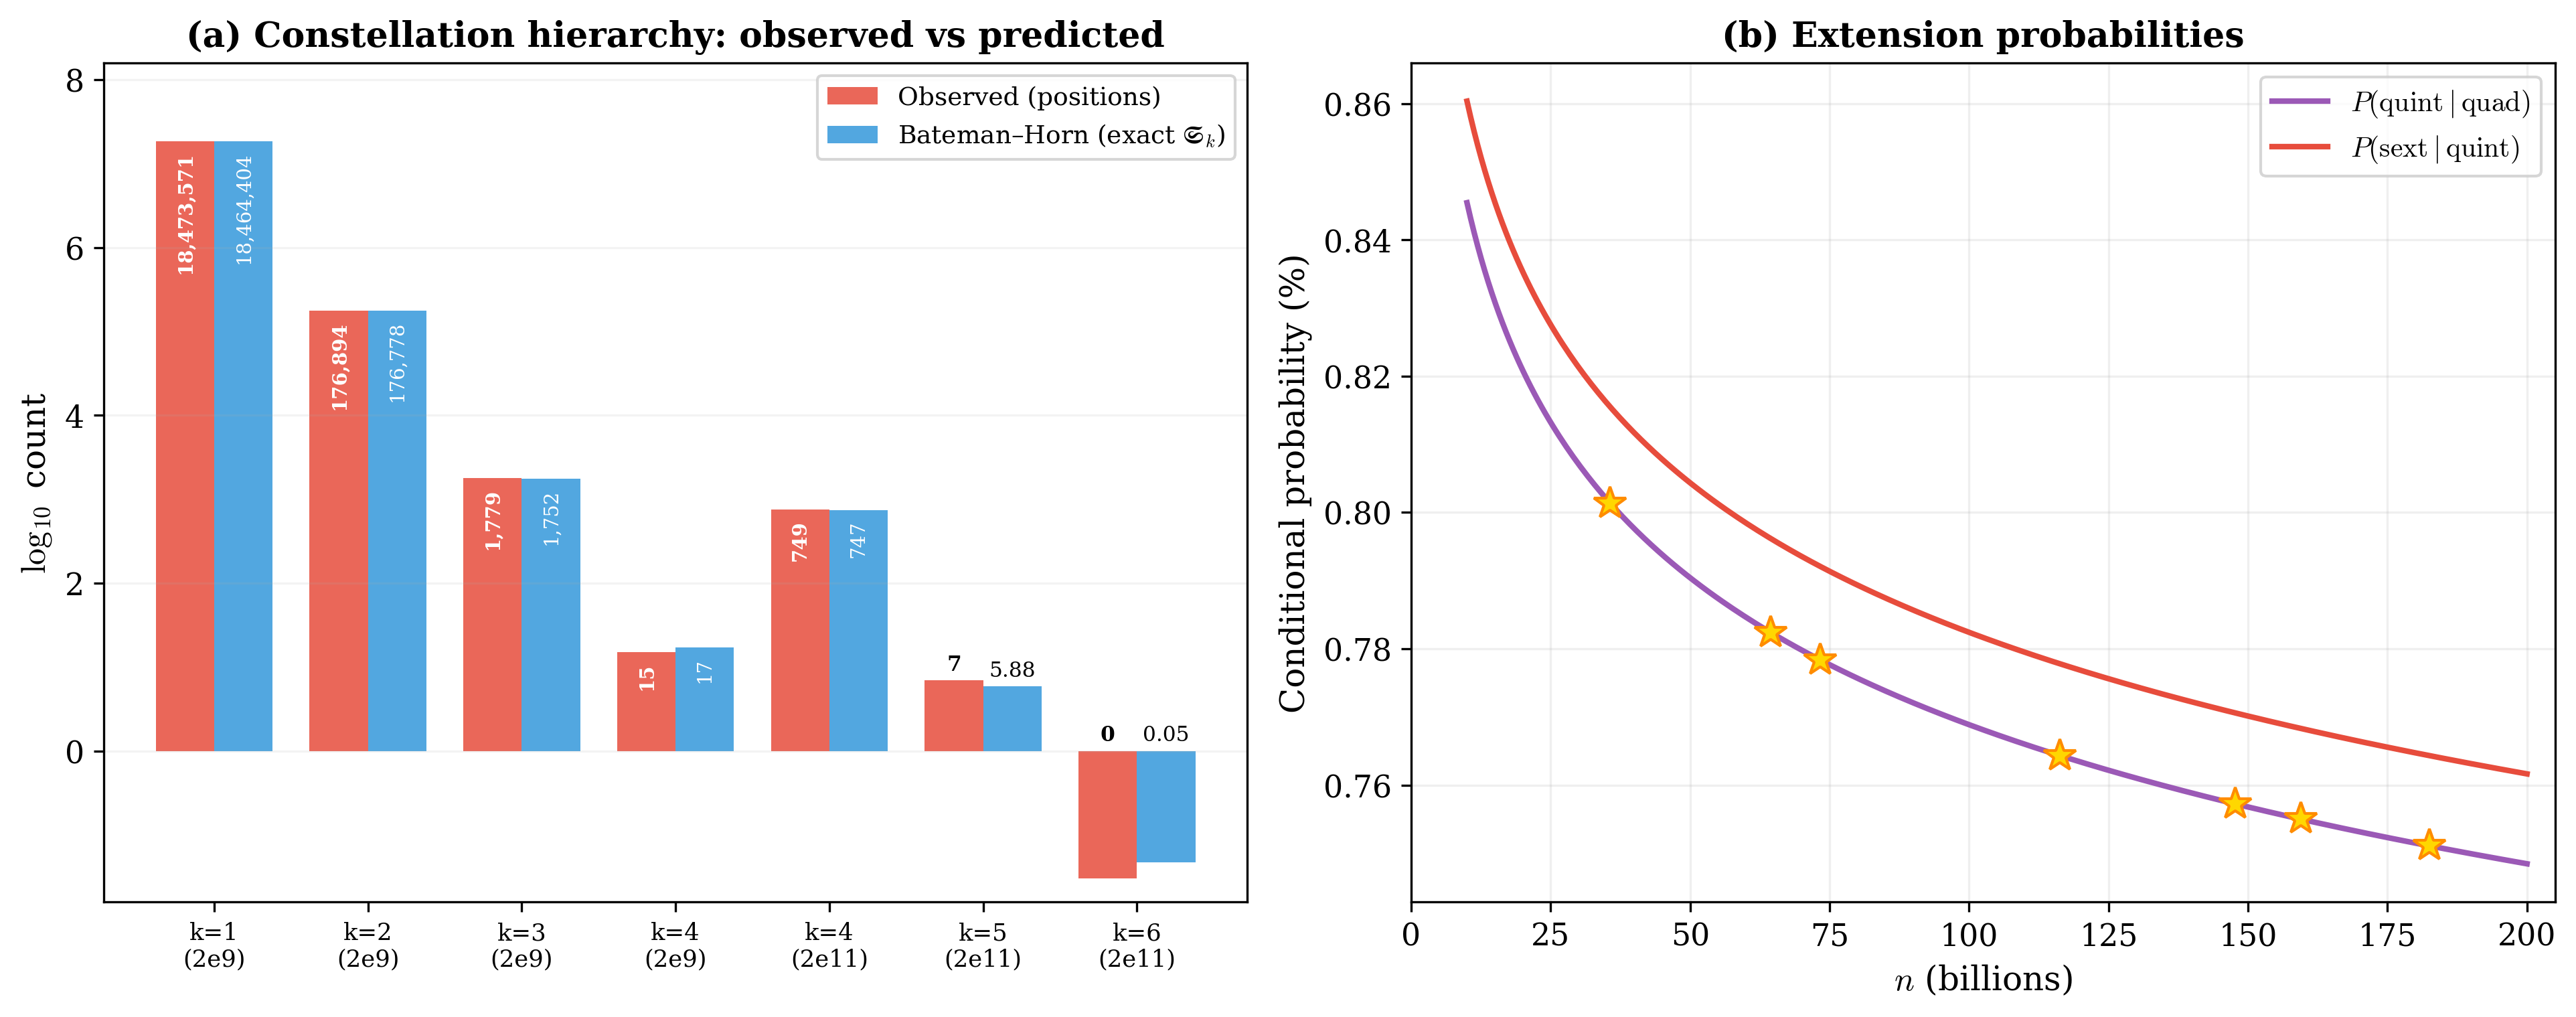
\includegraphics[width=\textwidth]{v2_fig2.png}
\caption{(a)~Observed position counts versus the parameter-free Bateman--Horn
prediction for $k = 1, \ldots, 6$ (log scale; the first four bars refer to the
pioneer zone, the last three to the full range).
(b)~Conditional extension probabilities
$P(\text{quint}\,|\,\text{quad}) = (\Sk{5}/\Sk{4})/\ln Q(n{+}4)$ and
$P(\text{sext}\,|\,\text{quint})$; stars mark the 7 quintuplets.}\label{fig:staircase}
\end{figure}

%==========================================================================
\section{The Seven Quintuplets}\label{sec:quintuplets}
%==========================================================================

\subsection{Catalog}

Table~\ref{tab:quints} lists all 7 prime quintuplets.  The digit counts are the
exact lengths of $Q(n)$ (they are one larger than in Version~1 and in the Part~II
catalogue, which reported $\lfloor \log_{10} Q(n) \rfloor$ instead of
$\lfloor \log_{10} Q(n) \rfloor + 1$); within each quintuplet all five values
have the same number of digits.

\begin{table}[H]
\centering
\caption{All 7 prime quintuplets for $Q(n)$ in $n \leq 2 \times 10^{11}$.
``Rank'' is the position in the sorted list of 742 quadruplets.}\label{tab:quints}
\smallskip
\begin{tabular}{clcccc}
\toprule
\# & Starting $n$ & Digits of $Q$ & $n/10^{11}$ & Quad rank & Gap from previous \\
\midrule
1 & 35\,676\,017\,721  & 488 & 0.357 & \#154 & --- \\
2 & 64\,482\,563\,907  & 499 & 0.645 & \#251 & 28.8\,B \\
3 & 73\,292\,417\,435  & 502 & 0.733 & \#284 &  8.8\,B \\
4 & 116\,255\,850\,744 & 511 & 1.163 & \#444 & 43.0\,B \\
5 & 147\,743\,683\,226 & 516 & 1.477 & \#570 & 31.5\,B \\
6 & 159\,430\,471\,996 & 517 & 1.594 & \#611 & 11.7\,B \\
7 & 182\,501\,065\,420 & 520 & 1.825 & \#681 & 23.1\,B \\
\bottomrule
\end{tabular}
\end{table}

\subsection{Spatial Distribution}

The quintuplets span the full search range: one in $[0, 50\text{B})$, two each
in $[50, 100)$, $[100, 150)$ and $[150, 200)$ billion (Figure~\ref{fig:field}).
The six gaps range from 8.8 to 43.0~billion (mean 24.5\,B, sample standard
deviation 12.8\,B).  A Kolmogorov--Smirnov test of the seven positions against
the Bateman--Horn cumulative distribution (proportional to $I_5(n)$) gives
$D = 0.265$, $p = 0.62$; against a uniform distribution on $[0, 2\times10^{11}]$
it gives $D = 0.180$, $p = 0.95$ (the value quoted in Version~1 corresponds to the
latter).  With seven points neither test has power to detect anything but gross
clustering; the data are simply consistent with the model.

\begin{figure}[htbp]
\centering
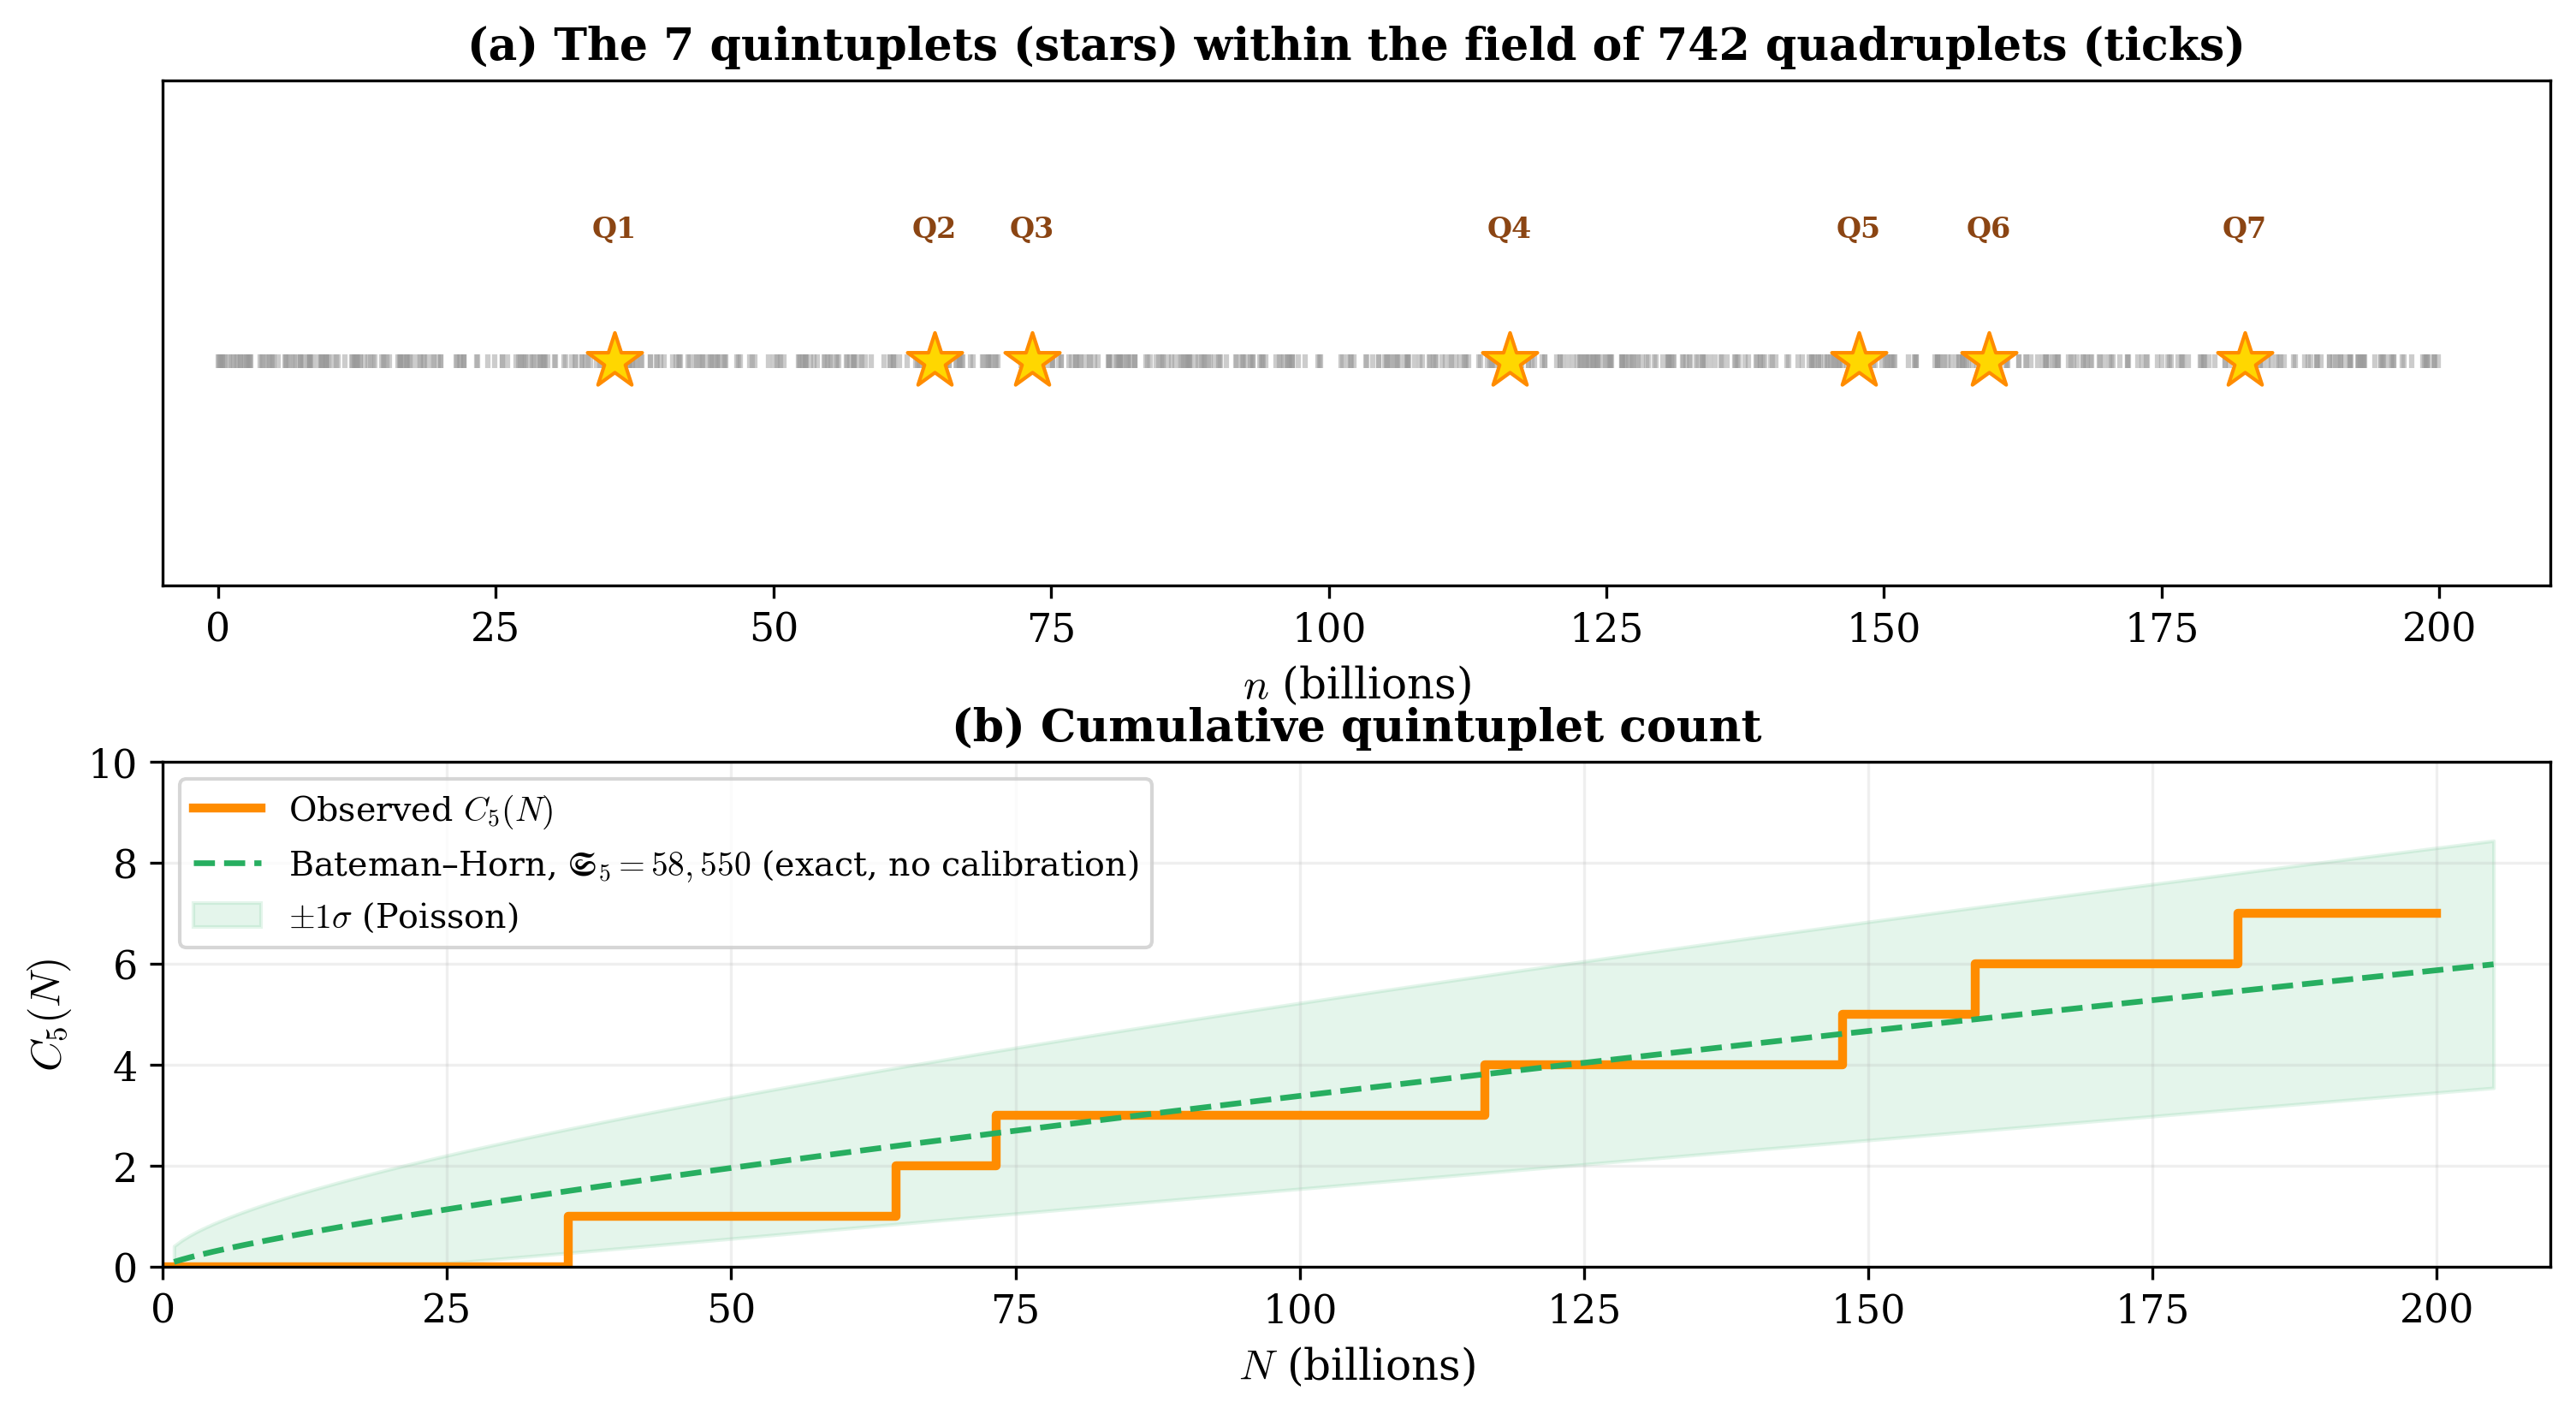
\includegraphics[width=\textwidth]{v2_fig1.png}
\caption{Top: quintuplet positions ($\bigstar$) within the 742-quadruplet field.
Bottom: cumulative count $C_5(N)$ versus the parameter-free Bateman--Horn curve
with $\Sk{5} = 58{,}550$ and its Poisson $\pm 1\sigma$ band.}\label{fig:field}
\end{figure}

%==========================================================================
\section{The Conditional Extension Model}\label{sec:conditional}
%==========================================================================

Given a quadruplet starting at~$n$, the conditional probability that it extends
to a quintuplet is
\begin{equation}\label{eq:cond}
  P(\text{quint}\,|\,\text{quad at } n) \approx
  \frac{\Sk{5}}{\Sk{4}} \cdot \frac{1}{\ln Q(n{+}4)}
  = \frac{8.99}{46 \ln n + \ln 47}.
\end{equation}
Summing \eqref{eq:cond} over the 742 catalogued quadruplets
($\langle \ln n \rangle = 24.90$) gives
\begin{equation}\label{eq:Equint}
  E_{\mathrm{cond}}[C_5] = \sum_{i=1}^{742} \frac{8.99}{\ln Q(n_i{+}4)} = 5.82,
\end{equation}
to be compared with the direct integral $E[C_5] = \Sk{5} I_5 = 5.88$ (the small
difference reflects the Poisson scatter of the quadruplet positions themselves).
The observed 7 lies inside the $1\sigma$ interval $[3.5, 8.3]$ of a Poisson
variable with mean 5.88, and $P(C_5 \geq 7 \,|\, 5.88) = 0.37$.
Under na\"{\i}ve independence ($\Sk{5}/\Sk{4} = 1$) one would expect only
$0.65$ quintuplets; the factor of~9 is entirely the singular-series ratio,
i.e.\ the fact that a quadruplet has already ``paid'' the sieve cost of the
resonant primes for four of the five positions.

%==========================================================================
\section{The Sextuplet Boundary}\label{sec:sextuplet}
%==========================================================================

At $N = 2 \times 10^{11}$,
\begin{equation}
  E[C_6] = \Sk{6}\, I_6(2 \times 10^{11}) = 535{,}500 \times 8.80 \times 10^{-8} = 0.047,
\end{equation}
so the probability of at least one sextuplet in the present range is
$1 - e^{-0.047} = 4.6\%$: its absence is the expected outcome.
Solving $E[C_6(N^*)] = 1$ gives
\begin{equation}
  \boxed{N^* \approx 1.03 \times 10^{13}}
\end{equation}
($1.01 \times 10^{13}$ with the $(46 \ln t)^6$ convention of Version~1), a
$52$-fold extension of the current search, where $Q(n)$ has 601 digits.
Table~\ref{tab:prediction} and Figure~\ref{fig:prediction} give the outlook.

\begin{table}[H]
\centering
\caption{Predicted counts (exact singular series, Eq.~\eqref{eq:BH}).}\label{tab:prediction}
\smallskip
\begin{tabular}{rccc l}
\toprule
Search bound $N$ & $E[C_5]$ & $E[C_6]$ & $P(C_6 \ge 1)$ & Status \\
\midrule
$2 \times 10^{11}$ (current) & 5.9 & 0.047 & 4.6\% & 7 / 0 observed \\
$10^{12}$ & 21 & 0.16 & 15\% & \\
$2 \times 10^{12}$ & 38 & 0.28 & 24\% & \\
$5 \times 10^{12}$ & 80 & 0.57 & 43\% & coin flip \\
$10^{13}$ & 141 & 0.98 & 62\% & \\
$\boldsymbol{1.03 \times 10^{13}}$ & $\boldsymbol{145}$ & $\boldsymbol{1.00}$ & $\boldsymbol{63\%}$ & \textbf{sextuplet boundary} \\
$2 \times 10^{13}$ & 251 & 1.69 & 82\% & \\
$5 \times 10^{13}$ & 538 & 3.52 & 97\% & \\
$10^{14}$ & 961 & 6.15 & 99.8\% & sextuplets routine \\
\bottomrule
\end{tabular}
\end{table}

\begin{figure}[htbp]
\centering
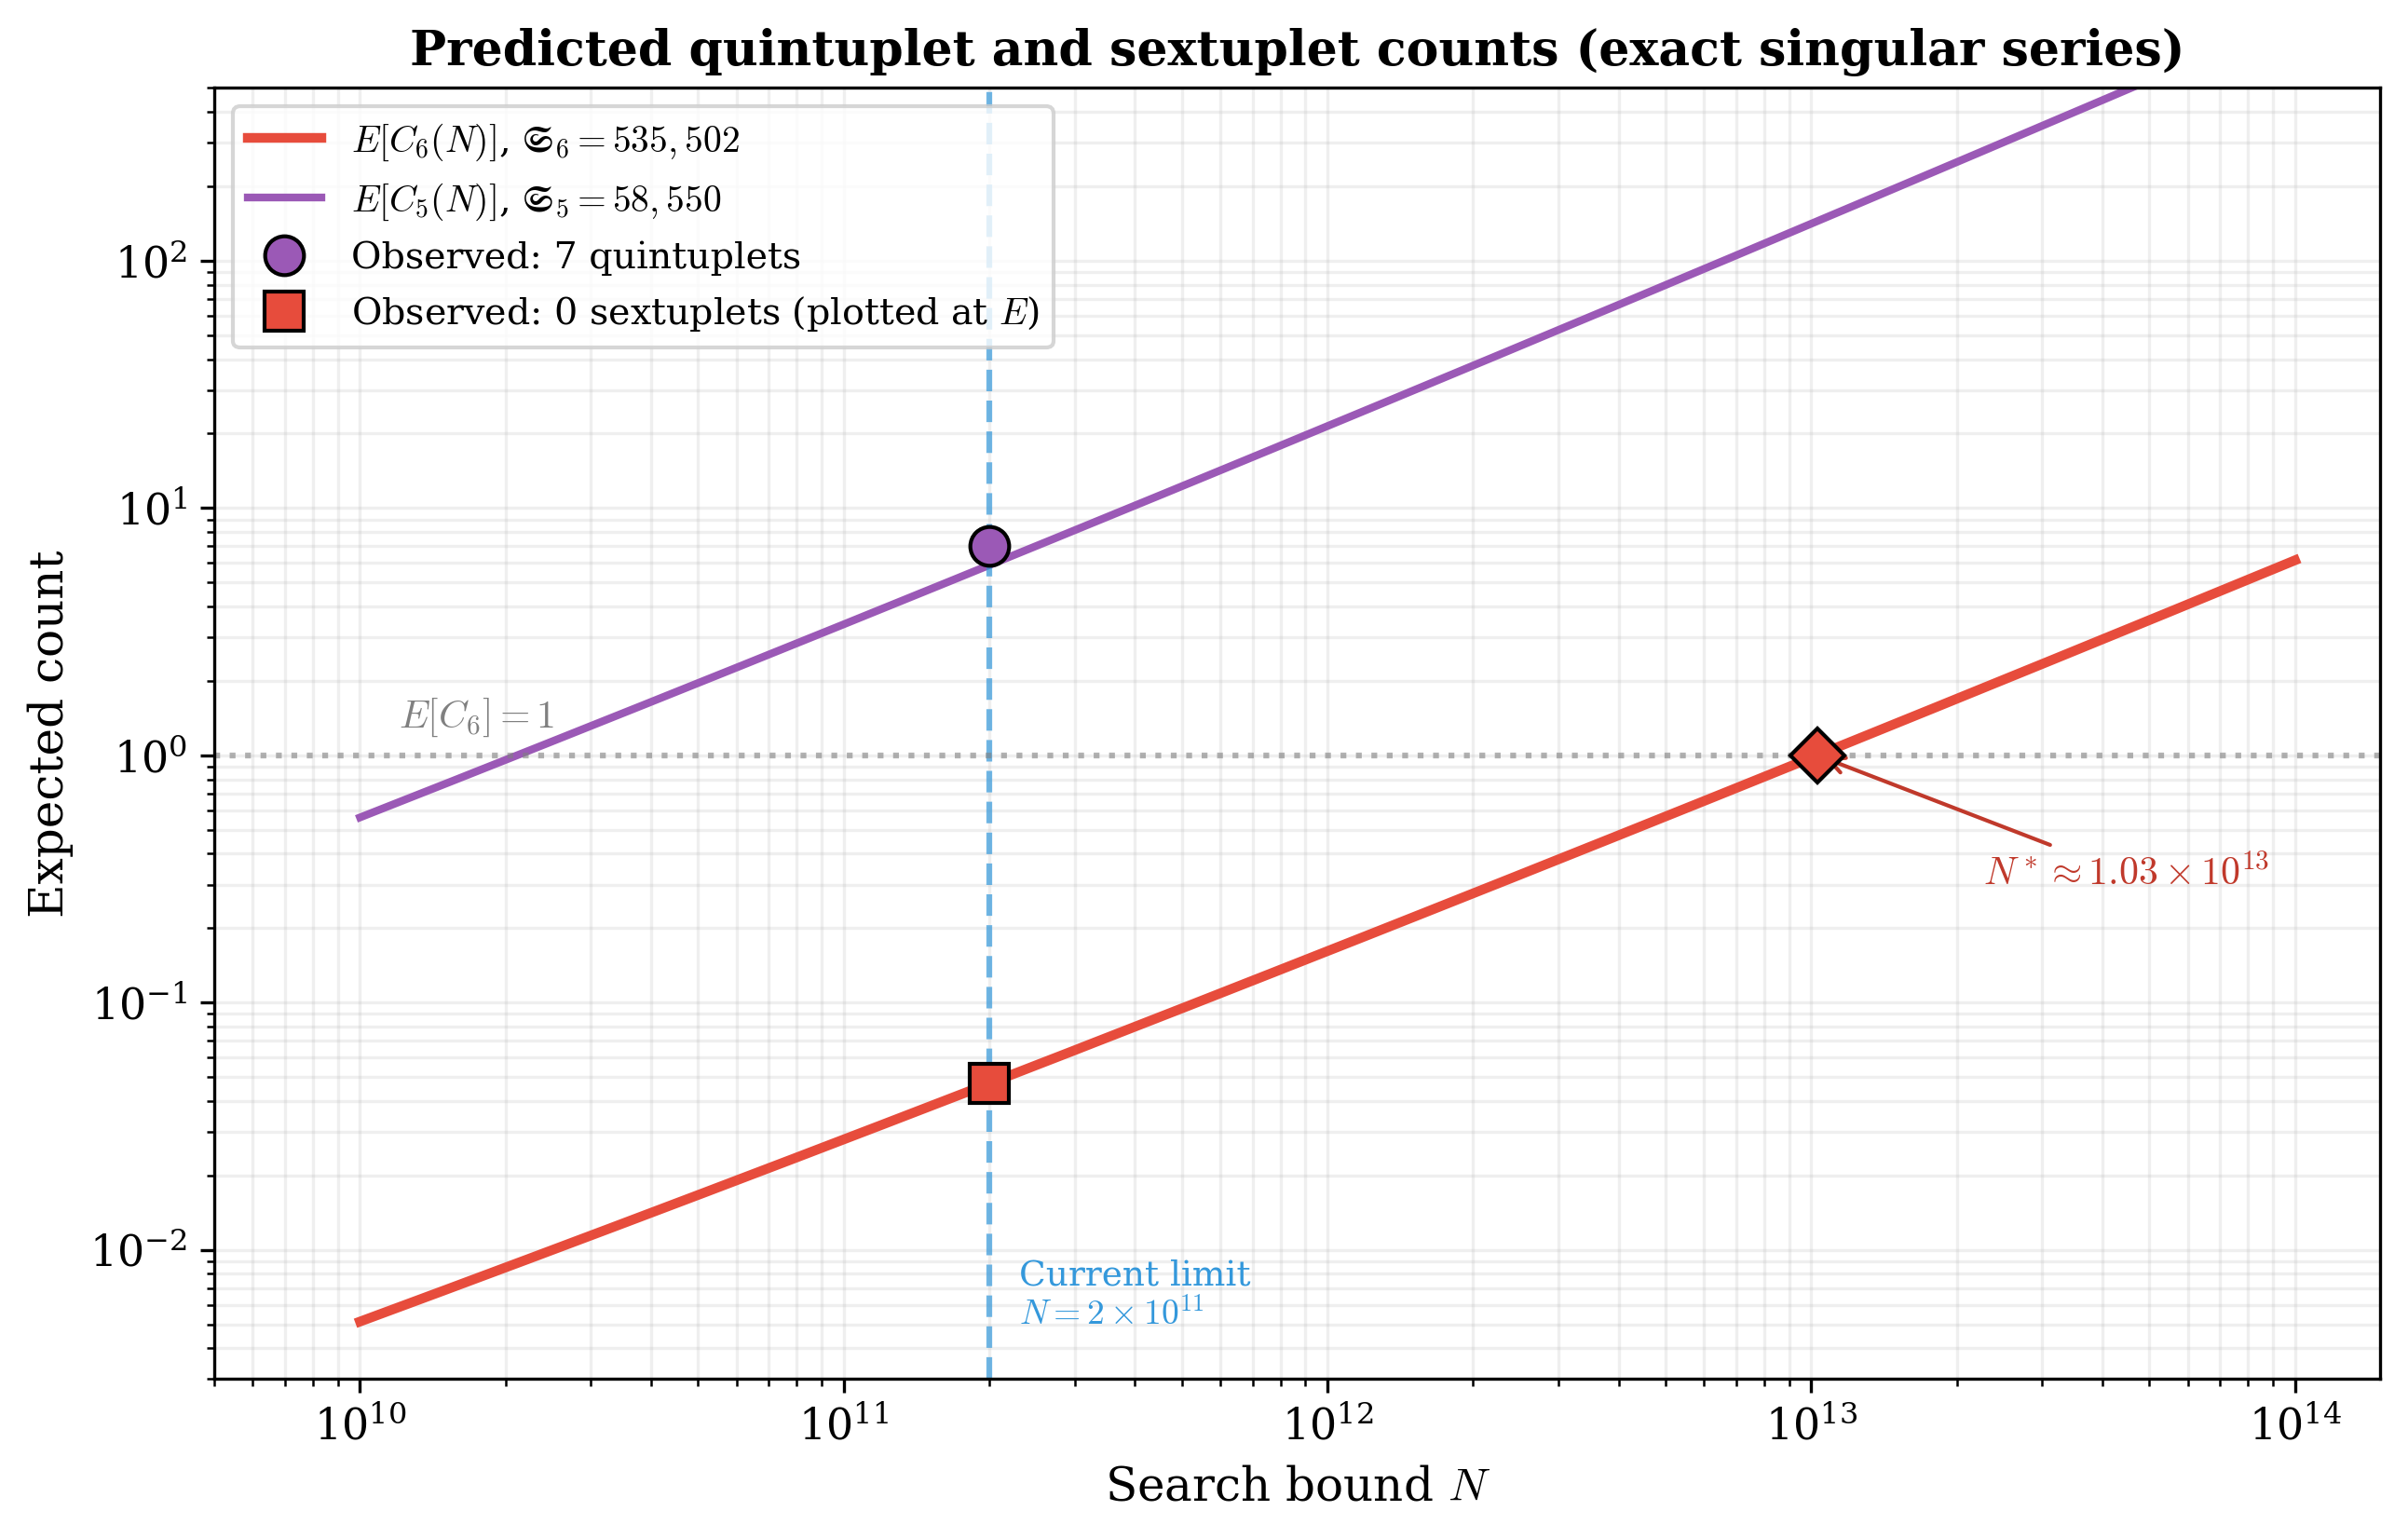
\includegraphics[width=0.92\textwidth]{v2_fig3.png}
\caption{$E[C_5(N)]$ and $E[C_6(N)]$ versus search bound.
The diamond marks the sextuplet boundary.}\label{fig:prediction}
\end{figure}

%==========================================================================
\section{The Suppression Factor}\label{sec:suppression}
%==========================================================================

The ratio of successive position counts is, by \eqref{eq:BH},
\begin{equation}\label{eq:R}
  R_{k \to k+1}(N) = \frac{E[C_k(N)]}{E[C_{k+1}(N)]}
  = \frac{I_k(N)}{I_{k+1}(N)} \Big/ \frac{\Sk{k+1}}{\Sk{k}}
  \approx \frac{46 \ln N_{\mathrm{eff}} + \ln 47}{9.0},
\end{equation}
where $N_{\mathrm{eff}}$ is a logarithmic mean of the range.  The factor is
therefore \emph{not} a universal constant (as Version~1 claimed) but grows
logarithmically with the search bound: Table~\ref{tab:suppression}.

\begin{table}[H]
\centering
\caption{Inter-level suppression factors: Bateman--Horn prediction \eqref{eq:R}
versus observed ratios of position counts.}\label{tab:suppression}
\smallskip
\begin{tabular}{llcc}
\toprule
Range & Transition & Predicted $R$ & Observed $R$ \\
\midrule
$N = 2\times10^{9}$  & $1 \to 2$ & 104.4 & 104.4 \\
                     & $2 \to 3$ & 100.9 &  99.4 \\
                     & $3 \to 4$ & 103.1 & 118.6 \\
                     & $4 \to 5$ & 103.0 & --- \\
$N = 2\times10^{11}$ & $3 \to 4$ & 126.9 & --- \\
                     & $4 \to 5$ & 127.1 & 107.0 \\
                     & $5 \to 6$ & 124.7 & --- \\
\bottomrule
\end{tabular}
\end{table}

The pioneer-zone ratios cluster around~$103$ and the full-range ratios around
$126$, exactly as \eqref{eq:R} predicts from $\ln(2\times10^{11})/\ln(2\times10^{9})$;
the two observed outliers ($118.6$ and $107.0$) involve counts of 15 and 7 and
are within Poisson noise.  The near-equality of the ratios
$\Sk{k+1}/\Sk{k} \approx 9$ at every level is what makes the factor almost
independent of~$k$ at fixed~$N$.

%==========================================================================
\section{Discussion}
%==========================================================================

\subsection{The Bifurcated Sieve}

The periodic obstruction at $p \equiv 1 \pmod{47}$ is a property of the
cyclotomic structure, not of the exponent~47 alone: for
$D_q(n) = n^q - (n{-}1)^q = \Phi_q(n, n{-}1)$ with any prime~$q$, every prime
factor of every value is $\equiv 1 \pmod q$, $\omega_1(p) = q - 1$ for
$p \equiv 1 \pmod q$ and zero otherwise, and the singular series is given by
\eqref{eq:accel} with the $L$-values modulo~$q$.  Larger~$q$ gives a longer
unobstructed corridor (no root below the first prime $\equiv 1 \pmod q$) and
hence larger constants, but also a smaller density $1/(q{-}1)$ of resonant
primes with individually more destructive cliffs.

\subsection{Quintuplets as a Bateman--Horn Prediction}

The 7 observed quintuplets match the parameter-free prediction $E = 5.88$
within $0.5\sigma$, and the conditional model gives $5.82$.  Together with the
$0.05\%$ and $0.07\%$ agreements for primes and pairs in the pioneer zone
(Table~\ref{tab:hierarchy}), this is a precise validation of Bateman--Horn for a
system of six polynomials of degree~46 at ${\sim}500$-digit scale.

\subsection{Sextuplet Outlook}

Part~II reports ${\sim}240$ CPU-core-hours for the range $2 \times 10^{11}$
\cite{Chen2026b}.  Reaching $N^* \approx 1.03 \times 10^{13}$ multiplies the
range by~52 and the per-candidate cost by roughly $(601/500)^{1.6} \approx 1.3$
for 600-digit modular arithmetic, i.e.\ ${\sim}16{,}000$ core-hours or about
four weeks on a 26-core workstation---feasible.  (Version~1's ``12{,}500
core-hours, 2 weeks'' omitted the digit-size factor and misconverted the hours.)
Note that at $N^*$ the \emph{expected} number of sextuplets is one; the
probability of actually having found one is $63\%$ (50\% is reached at
$N \approx 6.5 \times 10^{12}$), and reaching $90\%$ requires
$N \approx 2.9 \times 10^{13}$.

%==========================================================================
\section{Conclusion}
%==========================================================================

$Q(n) = n^{47} - (n{-}1)^{47}$ is the homogenised cyclotomic polynomial
$\Phi_{47}(n, n{-}1)$: all its prime factors are $\equiv 1 \pmod{47}$, it has no
roots modulo non-resonant primes and 46 roots modulo every resonant prime.
This bifurcated structure makes the Bateman--Horn Euler product oscillate
strongly, but factoring out $\prod_{\chi \ne \chi_0} L(1,\chi) = 0.11517$ yields
exact singular series $\Sk{4} = 6{,}514$, $\Sk{5} = 58{,}550$,
$\Sk{6} = 535{,}500$.  Without any calibration these reproduce the whole
observed hierarchy, from $18.47$ million primes in the pioneer zone ($0.05\%$)
to 749 quadruplet positions ($0.3\%$), 7 quintuplets ($E = 5.9$) and 0
sextuplets ($E = 0.047$) in the full range.  The first sextuplet is expected
near $N^* \approx 1.0 \times 10^{13}$, and the inter-level suppression factor
grows as $\approx 46 \ln N / 9$, from ${\approx}103$ in the pioneer zone to
${\approx}127$ at the present frontier.

%==========================================================================
\section*{Data and Code Availability}
%==========================================================================

Complete data and code for this paper:
\begin{center}
\url{https://github.com/Ruqing1963/Q47-Quintuplet-Sextuplet-Boundary}
\end{center}
\noindent The Version~2 material consists of:
\begin{itemize}[nosep]
  \item \texttt{compute\_singular\_series\_v2.py} --- plain and $L$-function evaluation of $\Sk{k}$;
  \item \texttt{predictions\_v2.py} --- all predictions, tests and tables;
  \item \texttt{generate\_figures\_v2.py} --- Figures 1--5;
  \item the corresponding \texttt{data/*\_v2.csv} files and \texttt{CHANGELOG\_v2.md}.
\end{itemize}
\noindent Quadruplet census data (Part~II):
\begin{center}
\url{https://github.com/Ruqing1963/Q47-Deep-Space-Quadruplet-Census}
\end{center}
\noindent Zenodo archives: \\
Part~III, this paper, Version~2: \url{https://doi.org/10.5281/zenodo.23178170} \\
Part~III, Version~1: \url{https://doi.org/10.5281/zenodo.18728917} \\
Part~II: \url{https://zenodo.org/records/18728540} \\
Part~I: \url{https://zenodo.org/records/18701355}

%==========================================================================
\begin{thebibliography}{99}
%==========================================================================

\bibitem{BatemanHorn1962}
P.\,T. Bateman and R.\,A. Horn,
``A heuristic asymptotic formula concerning the distribution of prime numbers,''
\textit{Math.\ Comp.}, vol.~16, no.~79, pp.~363--367, 1962.

\bibitem{HardyLittlewood1923}
G.\,H. Hardy and J.\,E. Littlewood,
``Some problems of `Partitio Numerorum'; III,''
\textit{Acta Math.}, vol.~44, pp.~1--70, 1923.

\bibitem{BirkhoffVandiver1904}
G.\,D. Birkhoff and H.\,S. Vandiver,
``On the integral divisors of $a^n - b^n$,''
\textit{Ann.\ of Math.}, vol.~5, no.~4, pp.~173--180, 1904.

\bibitem{Washington1997}
L.\,C. Washington,
\textit{Introduction to Cyclotomic Fields}, 2nd ed., Springer GTM~83, 1997.

\bibitem{Chen2026a}
R.\,Chen,
``Statistical Morphology and Geodesic Rigidity of Prime Constellations in
the Polynomial $Q(n) = n^{47} - (n-1)^{47}$:
A Complete Census of the First 2 Billion Cases,''
Zenodo, 2026. \url{https://zenodo.org/records/18701355}.

\bibitem{Chen2026b}
R.\,Chen,
``A Complete Census of Prime Quadruplets for
$Q(n) = n^{47} - (n-1)^{47}$ in the Range $1 \leq n \leq 2 \times 10^{11}$,''
Zenodo, 2026. \url{https://zenodo.org/records/18728540}.

\bibitem{Chen2026c}
R.\,Chen,
``Prime Quintuplets and the Sextuplet Boundary for $Q(n) = n^{47} - (n-1)^{47}$,''
Version~1, Zenodo, February 2026, \url{https://doi.org/10.5281/zenodo.18728917};
Version~2, October 2026, \url{https://doi.org/10.5281/zenodo.23178170}.

\bibitem{GMP}
GMP: The GNU Multiple Precision Arithmetic Library, \url{https://gmplib.org/}.

\bibitem{CrandallPomerance2005}
R. Crandall and C. Pomerance,
\textit{Prime Numbers: A Computational Perspective}, 2nd ed., Springer, 2005.

\bibitem{Maynard2015}
J. Maynard, ``Small gaps between primes,''
\textit{Ann.\ of Math.}, vol.~181, no.~1, pp.~383--413, 2015.

\bibitem{GreenTao2008}
B. Green and T. Tao, ``The primes contain arbitrarily long arithmetic progressions,''
\textit{Ann.\ of Math.}, vol.~167, pp.~481--547, 2008.

\end{thebibliography}

\end{document}
